\documentclass[notitlepage]{article}

\usepackage{bibunits}
\usepackage{comment}
\usepackage{graphicx}
\usepackage{amsmath}
\usepackage{amssymb}
\usepackage{datetime}
\usepackage{numprint}

% processes above options
\usepackage{palatino}  %OR newcent ncntrsbk helvet times palatino
\usepackage{url}
\usepackage{footmisc}
\usepackage{endnotes}
\usepackage{graphicx}
\usepackage{fancyvrb}
\usepackage{varwidth}

\setcounter{secnumdepth}{5}
\begin{document}

\nplpadding{2}
\newdateformat{isodate}{
  \THEYEAR -\numprint{\THEMONTH}-\numprint{\THEDAY}}
  
\title{Algorithm Abstraction - Exam 1}
\author{}
\date{\isodate\today}

\maketitle

\tableofcontents


\newpage
 

 \section{Chapter 1: Representative Problems and Gale-Shapley}
        \subsection{Stable Matching Definitions}
            \begin{itemize}
                \item \textbf{Algorithm}: A procedure that takes an input, transforms it, and then outputs the result
                \item \textbf{Unstable Matching}: A matching such that there exists a pair $(x_1,y_1)$ in matching M where
                    both $x_1$ and $y_1$ both prefer another partner to the one they currently have (unstable pair)
                \item \textbf{Stable Matching}: A matching such that there are \textbf{NO} unstable pairs 
                \item \textbf{Perfect Matching}: A matching where every element of Set A is matched with exactly
                    one element of set B
            \end{itemize}
        \subsection{Gale-Shapley}
            \textbf{Gale-Shapley}: Algorithm that is guaranteed to find the same perfect matching
            and a stable matching every time
\begin{center}          
     \begin{BVerbatim}
GALE–SHAPLEY (preference lists for hospitals and students)
    INITIALIZE M to empty matching.
    WHILE (some hospital h is unmatched and hasn’t proposed to every student)
        s ← first student on h’s list to whom h has not yet proposed.
    IF (s is unmatched)
        Add h–s to matching M.
    ELSE IF (s prefers h to current partner h')
        Replace h'-s with h-s in matching M.
    ELSE
        s rejects h.
    RETURN stable matching M.
    \end{BVerbatim}
\end{center}      

 \section{Chapter 2: Algorithm Analysis}
    \subsection{Big O Notation}
        \begin{itemize}
            \item  The upper bound of a function such that $f(n)$ is $O(g(n))$ if 
            there exists constants $c > 0$ and $n_0 \geq 0$ such that $ 0 \leq f(n) \leq c * g(n)$ for
            all $n \geq n_0$ \\
            \item Can be further expanded such that $f(n)$ is $O(g(n))$ if 
            $$\lim\limits_{n \to \infty} \frac{f(n)}{g(n)} = 0$$
            \item if $f_1$ is $O(g_1)$ and $f_2$ is $O(g_2)$, then $f_1f_2$ is $O(g_1g_2)$
            \item if $f_1$ is $O(g_1)$ and $f_2$ is $O(g_2)$, then $f_1+f_2$ is $O(max\{ g_1, g_2\})$
        \end{itemize}
    \subsection{Big Omega($\Omega$) Notation}
        \begin{itemize}
            \item The lower bound of a function such that $f(n)$ is $\Omega(g(n))$ if 
                there exists constants $c > 0$ and $n_0 \geq 0$ such that $ 0 \leq c * g(n) \leq f(n)$
                for all $n \geq n_0$ \\
            \item Can be further expanded such that $f(n)$ is $\Omega(g(n))$ if 
                $$\lim\limits_{n \to \infty} \frac{g(n)}{f(n)} = 0$$
        \end{itemize}
    \subsection{Big Theta($\Theta$) Notation}
        \begin{itemize}
            \item The tight bound of a function such that $f(n)$ is $\Theta(g(n))$ if 
                there exists constants $c_1 > 0$, $c_2 > 0$, and $n_0 \geq 0$ such 
                that $ 0 \leq c_1*g(n) \leq f(n) \leq c_2*g(n)$  for all $n \geq n_0$ \\
            \item Can be further expanded such that $f(n)$ is $\Theta(g(n))$ if 
                $$\lim\limits_{n \to \infty} \frac{f(n)}{g(n)} = c$$
        \end{itemize}

 \section{Chapter 3: Graphs}
    \subsection{Graph Types and Definitions}
    \begin{itemize}
        \item \textbf{Undirected Graphs}: Set of nodes (vertices) and bidirectional edges between nodes
        \item \textbf{Directed Graphs}: Set of nodes and directional edges between nodes
        \item \textbf{Adjacency Matrix}: n-by-n matrix where $A_{uv} = 1$ if (u,v) is an edge
        \item \textbf{Adjacency Lists}: Node-indexed array of lists with only edges in the list
        \item \textbf{Path}: There is a path between two nodes if there is a sequence of edges and nodes
            that go from one node to another
        \item \textbf{Simple Path}: All nodes in the path are distinct
        \item \textbf{Connected Graph}: A graph is connected if there is a path for every pair of nodes
        \item \textbf{Cycles}: A cycle is a path $v_1,v_2,...,v_k$ in which $v_1=v_k$ and $k \geq 2$
        \item \textbf{Tree}: An undirected graph is a tree if its connected and does not contain a cycle
    \end{itemize}
    
    \subsection{Connectivity and Traversal}
    \begin{itemize}
        \item \textbf{Breadth-First Search}: Explore outward from starting node s in all possible directions
            one layer at a time. Runs in O(m+n) if graph is given as adjacency list
    \end{itemize}
    
    \subsection{Bipartite Graphs}
    \begin{itemize}
        \item \textbf{Bipartite Graphs}: An undirected graph is bipartite if the nodes can be colored blue or
            white such that every edge has one white and one blue end
        \item If graph G is bipartite, it cannot contain an odd-length cycle
    \end{itemize}

    \subsection{DAGs and Topological Orderings}
    \begin{itemize}
        \item \textbf{Directed Acyclic Graph (DAG)}: A DAG is a directed graph that contains no directed
            cycles
        \item \textbf{Topological Order}: An ordering of a directed graph such that for nodes $v_1,v_2,...v_n$ 
            and every edge $(v_i, j_2)$, we have $i < j$
\begin{verbatim}
* Maintain the following information:
    - count(w) = remaining number of incoming edges
    - S = set of remaining nodes with no incoming edges
* Initialization: O(m + n) via single scan through graph.
* Update: to delete v
    -remove v from S
    - decrement count(w) for all edges from v to w; 
        and add w to S if count(w) hits 0
    - this is O(1) per edge
\end{verbatim}
        \item if G has a Topological Order, then G is a DAG            
    \end{itemize}

 \section{Chapter 4 - Greedy Algorithms (1)}
    \subsection{Coin Change}
    \begin{itemize}
        \item Given a currency, find a way for a cashier to give the customer the fewest possible number of coins
        \item \textbf{Cashiers Algorithm}: At each iteration, add coin of the largest value possible that does not take
            us past the remaining amount to be paid
        \item Cashiers Algorithm is not always optimal depending on the denomination of coins present
    \end{itemize}
    
    \subsection{Interval Scheduling}
    \begin{itemize}
        \item Job j starts at $s_j$ and finishes at $f_j$
        \item Two jobs are compatible if they don't overlap
        \item Goal: Find maximum subset of mutually compatible jobs
        \item \textbf{Earliest-Finish-Time-First}
\begin{verbatim}
SORT jobs by finish times and renumber so that f1 <= f2 <= ... <= fn.
S <- 0 .
FOR j = 1 TO n
    IF (job j is compatible with S)
    S <- S U { j }.
RETURN S
\end{verbatim}
    \item Optimal algorithm that takes O(nlogn) time
    \end{itemize} 

    \subsection{Interval Partitioning}
    \begin{itemize}
        \item Goal: find minimum number of classrooms to schedule all lectures so that no 
            two lectures occur at the same time in the same room
        \item \textbf{Earliest-Start-Time-First Algorithm}
\begin{verbatim}
SORT lectures by start times and renumber so that s1 <= s2 <= ... <= sn.
d <- 0.
FOR j = 1 TO n
    IF (lecture j is compatible with some classroom)
        Schedule lecture j in any such classroom k.
    ELSE
        Allocate a new classroom d + 1.
        Schedule lecture j in classroom d + 1.
        d <- d + 1.
RETURN schedule
\end{verbatim}
    \item Can be implemented  in O(nlogn) time and is optimal
    \end{itemize}
    
    \subsection{Minimize Lateness}
    \begin{itemize}
        \item Single resource processes one job at a time
        \item Job j requires tj units of time and due at time dj
        \item if j starts at time sj, finishes at time fj = sj + tj
        \item Goal: Goal: schedule all jobs to minimize maximum lateness $L=max_jl_j$
        \item \textbf{Earliest-Deadline-First}
\begin{verbatim}
SORT jobs by due times and renumber so that d1 <=  d2 <= ... <= dn.
t <- 0.
FOR j = 1 TO n
    Assign job j to interval [t, t + tj ].
    sj <- t ; fj <- t + tj.
    t <- t + tj.
RETURN intervals [s1, f1], [s2, f2], ..., [sn, fn]
\end{verbatim}
    \item Earliest-Deadine-First Schedule S is optimal 
    \end{itemize}


    \subsection{Optimal Caching}
    \begin{itemize}
        \item \textbf{Cache Hit}: Item already in cache when requested
        \item \textbf{Cache Miss}: Item not already in cache when requested, must be brought into
            cache and evict some existing item if cache is full
        \item Goal: Eviction Schedule that minimizes number of cache misses
        \item A reduced schedule is a schedule that only inserts an item into the cache in a step in which
            that item is requested
        \item Farthest-in-Future is an optimal eviction algorithm in offline caching
        \item \textbf{Offline Algorithm}: Full sequence of request is known beforehand
        \item \textbf{Online Algorithm}: Full sequence of request is \textbf{NOT} known beforehand
        \item Some other caching methods are \textbf{LIFO} which evicts page brought in most recently and
            \textbf{LRU} which evicts page whose most recent access was earliest (FF with direction of time reversed)
    \end{itemize}
    
    \subsection{Dijkstras Algorithm}
    \begin{itemize}
        \item \textbf{Dijsktras Algorithm}: Algorithm to find the shortest possible path from starting
            point s to destination point t where the edge weights are greater than 0. \\
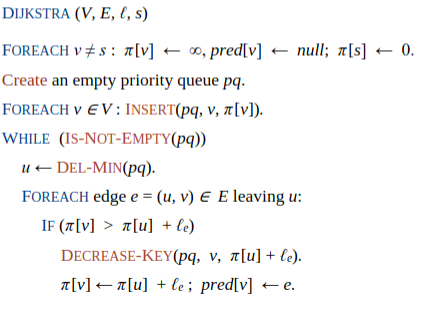
\includegraphics[width=3in]{/home/esteban/Desktop/school/fall2023/algo/studyGuides/exam1/dijkstra.png}
    \end{itemize}

    \subsection{Minimum Spanning Tree}
    \begin{itemize}
        \item \textbf{Cut}: A partition of nodes into two nonempty subsets S and V-S
        \item \textbf{Cutset}: Cutset of a cut S is the set of edges with exactly one endpoint in S
        \item \textbf{Spanning Tree}: Let H=(V,T) be a subgraph of an undirected graph G=(V,E). 
            H is a spanning tree of G is H is both acyclic and connected
        \item \textbf{Minimum Spanning Tree (MST)}: Given a connected, undirected graph G=(V,E) with edge costs $c_e$, a
            MST(V,T) is a spanning tree of G such that the sum of the edge costs in T is minimized. An edge is 
            in every MST if edge e is the cheapest edge crossing from S to complement V-S and e is in no MST
            if it is the most expensive edge on some cycle
    \end{itemize}

\end{document}
